\section{Problema}
%$\mathcal{G}$
%\emph{Clique}
\subsection{Motivación}
\begin{frame}%\frametitle{Motivación}
    \begin{block}{Motivación}
    \begin{itemize} 
    	\item Los servicios de fibra al hogar \emph{(Fiber-To-The-Home - FTTH)} tienen una gran penetración mundial brindando a los clientes finales transferencias de datos a altas velocidades.
    	\item La cantidad de aplicaciones y servicios sobre internet ha crecido exponencialmente.
    	\item Es mandatorio escalar de forma inteligente la infraestructura de red.
    	\item Dado que el despligue de la fibra optica es una importante inversión económica, el diseño topológico de las redes \emph{FTTH} debe continuar considerandose.
	\end{itemize} 
    \end{block}
    %\begin{center}
    %    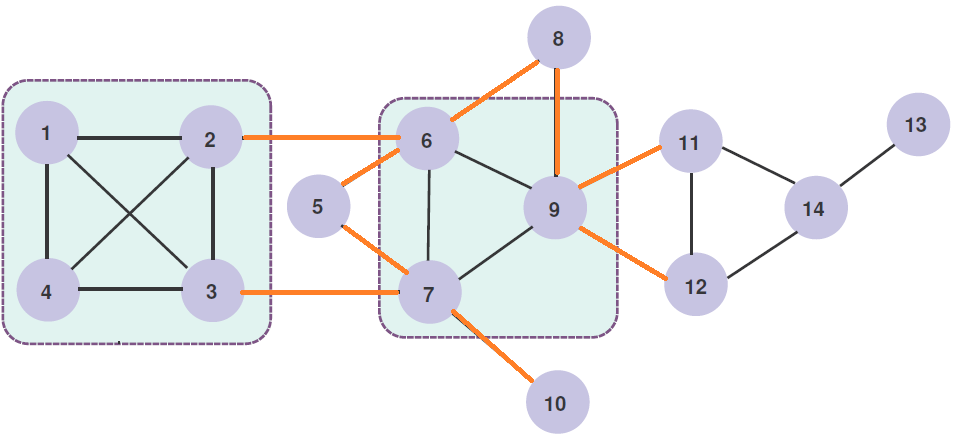
\includegraphics[scale=0.35]{figuras/martinsMod2}
    %\end{center}
\end{frame}

\subsection{Objetivos I}
\begin{frame}%\frametitle{Objetivos I}
    \begin{block}{Objetivos I}
	\begin{itemize} 
    	\item Problema de optimización combinatoria motivado por el diseño topológico de redes de comunicaciones 
con restricciones de confiabilidad.
		\item El objetivo es interconectar nodos distinguidos, llamados terminales, utilizando un nivel adecuado de redundancia y de forma simultanea, satisfacer las restricciones de confiabilidad.
	\item En el análisis de confiabilidad nos enfrentamos a fallas aleatorias en los componentes del sistema. Se considera el modelo como realista hostil, donde tanto nodos como aristas pueden fallar.
	\end{itemize} 
    \end{block}
\end{frame}

\subsection{Objetivos II}
\begin{frame}%\frametitle{Objetivos II}
    \begin{block}{Objetivos II}
	\begin{itemize} 
    	\item Encontrar una solución de costo mínimo que alcance un umbral de confiabilidad, donde tanto los nodos como los enlaces pueden fallar con probabilidades dadas.
		\item Entender el trade-off entre costo-confiabilidad, y como la confiabilidad aumenta naturalmente agregando niveles de redundancia entre los nodos terminales.
		\item Entender el impacto en la confiabilidad de las redes solución al aumentar o disminuir las probabilidades de falla elementales tanto en nodos como enlaces.
    	\item Pertenece a la clase de problemas \emph{NP-Hard}.
    	\item Se propone una solución que resuelve el problema de forma apróximada con una metodología \emph{GRASP/VND} para el problema de optimización y para el análisis de la confiabilidad el método \emph{RVR}.
	\end{itemize} 
    \end{block}
\end{frame}

\subsection{Definición}
\begin{frame}\frametitle{Generalized Steiner Problem with Node-Connectivity Constraints and
Hostile Reliability (GSPNCHR)}
    \begin{definition}[GSPNCHR]
Consider a simple undirected graph $G=(V,E)$, terminal-set $T \subseteq V$, link-costs $\{c_{i,j}\}_{(i,j) \in E}$ 
and connectivity requirements $R=\{r_{i,j}\}_{i,j \in T}$. Further, we assume that both links and non-terminal (Steiner) nodes 
fail with respective probabilities $P_E=\{p_e\}_{e\in E}$ and $P_{V-T}=\{p_v\}_{v\in V-T}$. 
Given a reliability threshold $p_{min}$, the goal is to build 
a minimum-cost topology $G_S \subseteq G$ meeting both the connectivity requirements 
$R$ and the reliability threshold: $R_{K}(G_S) \geq p_{min}$, being $K=T$ the terminal-set.
\end{definition}
\end{frame}

\subsection{Formulación como problema de programación matematica}
\begin{frame}\frametitle{GSPNCHR}
\begin{align}
\min &\sum_{(i,j)\in E} c_{i,j}x_{i,j} \notag \\
s.t. x_{ij}&\geq y_{(i,j)}^{u,v}+y_{(j,i)}^{u,v} \forall (i,j)\in E,
\forall u,v\in T, u \neq v \\
\sum_{(u,i)\in E}y_{(u,i)}^{u,v} &\geq r_{u,v} \, \, \forall \, u,v\in T, \, u\neq v \\
\sum_{(j,v)\in E}y_{(j,v)}^{u,v} &\geq r_{u,v} \, \, \forall \, u,v\in T, \, u\neq v \\
\sum_{(i,p)\in I(p)}y_{(i,p)}^{u,v}  - \sum_{(p,j)\in I(p)}y_{(p,j)}^{u,v}&\geq 0, \, \forall p\in V-\{u,v\}, \, \forall u,v\in T, \, u \neq v \notag \\
\end{align}
\end{frame}

\subsection{Formulación como problema de programación matematica}
\begin{frame}\frametitle{GSPNCHR}
\begin{align}
\sum_{(s,i)\in E} x_{s,i} &\leq M \hat{x}_{s}, \, \forall s\in V-T \\
R_{K}(G_S(\{x_{ij}\})) &\geq p_{min} \\
x_{(i,j)} &\in \{0,1\} \, \forall (i,j)\in E \\
\hat{x}_{i} &\in \{0,1\} \, \forall i \in V-T  \\
 y_{(i,j)}^{u,v} &\in \{0,1\} \, \forall (i,j)\in E, \, \forall u,v \in T, \, u \neq v
\end{align}
\end{frame}

\section{Resultados Teóricos}
\subsection{Resultados Teóricos}
\begin{frame}%\frametitle{}
    \begin{block}{Resultados Teóricos}
    \begin{small}
		\begin{itemize} 
    		\item Se demuestra la complejidad computacional del problema \emph{(NP-hardness)}.
			\item Se modela el problema para instancias particulares con $r_{ij} = k, k \geq 2$, tanto para arista conectividad como para nodo conectividad.
			\item Se encuentran cotas inferiores para las formulaciones anteriores aplicando teoría de dualidad y relajación lagrangiana.
	    	\item Formulación de programación matemática del problema para las versiones $k$ nodo-conectividad y $k$ arista-conectividad aplicando los teoremas de BienStock y Monma.
    		\item Se proponen algoritmos de orden polinomial para resolución del problema en forma exacta de casos particulares respecto a conectividad y topología de grafos.
    	\end{itemize} 
    			\end{small}
    \end{block}
\end{frame}

\section{Estado del arte}
\subsection{Trabajos Relacionados}
\begin{frame}\frametitle{}
\begin{block}{Trabajos Relacionados}
	\begin{itemize} 
    	\item Se dedicó un capítulo entero donde se expone el relevamiento del estado del arte de la temática de esta tesis: Confiabilidad en redes, Diseño topologico de redes, GRASP, VNS, RVR y otras como Crude Monte Carlo.
    	\item Son escasos los trabajos que abordan conjuntamente la optimización topológica de la red  bajo restricciones de confiabilidad.
    	\item VNS y RVR han sido utilizados con gran éxito en problemas de optimización combinatoria.
    \end{itemize} 
\end{block}
\end{frame}

\subsection{Publicación}
\begin{frame}\frametitle{}
\begin{block}{Publicación}
	\begin{enumerate}
		\begin{small}
			\item A GRASP/VND Heuristic for the Generalized Steiner Problem with Node-Connectivity Constraints and Hostile Reliability to be published in the Proceedings of the 8th International Conference on Variable Neighborhood Search (ICVNS March 2021). Khalifa University, Abu Dhabi, U.A.E. The article will be published by Springer in the Lecture Notes in Computer Science (LNCS) series.	
		\end{small}
	\end{enumerate}
\end{block}
\end{frame}

\section{Solución}
\subsection{Metodología}
\begin{frame}\frametitle{GRASP/VND}
\begin{block}{}
\begin{small}
\begin{itemize}
 \item Utilizamos una metodología GRASP/VND.
 \item GRASP y VND son metaheurísticas bien conocidas que se han utilizado con éxito para resolver muchos problemas difíciles de optimización combinatoria.
 \item GRASP es un poderoso proceso de arranque múltiple que opera en dos fases. Se construye una solución factible en una primera fase, cuyo vecindario luego se explora en la fase de búsqueda local.
 \item VND explora varias estructuras de vecindad en un orden determinista. Su éxito se basa en el simple hecho de que las diferentes estructuras de vecindad no suelen tener el mismo mínimo local. Así, la solución resultante es simultáneamente una solución localmente óptima en todas las estructuras vecinas.
\end{itemize} 
\end{small}
\end{block}
\end{frame}

\subsection{Esquema General}
\begin{frame}\frametitle{Esquema General}
    \begin{block}{Network Design}
\begin{algorithm}[H]
\floatname{algorithm}{Alg}
\caption{$sol = NetworkDesign(G_B,iter,k,p_{min},P_E,P_{V-T},simiter)$}
\begin{algorithmic}[1]
\begin{small}    
\STATE $i \leftarrow 0; \, P \leftarrow \emptyset; \, sol \leftarrow \emptyset$
\WHILE {$i < iter$}
\STATE $\overline{g} \leftarrow Construction(G_B,P,k)$
\STATE $g_{sol} \leftarrow VND(\overline{g},P)$
\STATE $reliability \leftarrow RVR(g_{sol},P_E,P_{V-T},simiter)$
\IF{$reliability > p_{min}$}
\STATE $sol \leftarrow sol \cup \{g_{sol}\}$
\ENDIF
\ENDWHILE
\RETURN $sol$
\end{small}
\end{algorithmic}
\end{algorithm}
    \end{block}
\end{frame}

\subsection{GRASP - Fase Construcción}
\begin{frame}\frametitle{}
    \begin{block}{}
\begin{algorithm}[H]
\floatname{algorithm}{Alg}
\caption{$(sol,P) = Construction(G_B,C,R,k)$}
\begin{algorithmic}[1]
\begin{scriptsize}
\STATE $g_{sol} \leftarrow (S_D^{(I)},\emptyset)$; $m_{i,j}\leftarrow r_{i,j}$; $P_{i,j}\leftarrow \emptyset, \forall i,j \in S_{D}^{(I)}$; $A_{i,j}\leftarrow 0, \forall i,j \in S_{D}^{(I)}$
\WHILE {$\exists \, m_{i,j}>0: A_{i,j}<MAXATTEMPTS$}
\STATE $(i,j) \leftarrow ChooseRandom(S_{D}^{(I)}: m_{i,j}>0)$
\STATE $\overline{G} \leftarrow G_B \setminus P_{i,j}$
\FORALL {$(u,v)\in E(\overline{G})$}
\STATE $\overline{c}_{u,v} \leftarrow c_{u,v} \times 1_{\{(u,v) \notin g_{sol}\}}$
\ENDFOR
\STATE $L_p \leftarrow KSP(k,i,j,\overline{G},\overline{C})$
\IF{$L_p=\emptyset$}
\STATE $A_{i,j} \leftarrow A_{i,j}+1$; $P_{i,j} \leftarrow \emptyset$; $m_{i,j}\leftarrow r_{i,j}$ 
\ELSE 
\STATE $p \leftarrow SelectRandom(L_p)$; $g_{sol} \leftarrow g_{sol} \cup \{p\}$
\STATE $P_{i,j} \leftarrow P_{i,j} \cup \{p\}$; $m_{i,j} \leftarrow m_{i,j}-1$
\STATE $(P,M) \leftarrow GeneralUpdateMatrix(g_{sol},P,M,p,i,j)$
\ENDIF
\ENDWHILE
\RETURN $(g_{sol},P)$
\end{scriptsize}    
\end{algorithmic}
\end{algorithm}
\end{block}
\end{frame}

\subsection{Fase Búsqueda Local}
\begin{frame}\frametitle{Fase Búsqueda Local}
\begin{block}{VND}
\begin{small}
El objetivo es combinar una rica diversidad de vecindades para obtener una solución óptima local para cada vecindario. NetworkDesign considera una implementación clásica de VND, ordenando las respectivas búsquedas locales después de la fase de construcción. Se consideran tres estructuras de vecindad para construir VND.
\begin{itemize}
 \item SwapKeyPathLocalSearch
 \item KeyPathLocalSearch
 \item KeyTreeLocalSearch
\end{itemize} 
\end{small}
\end{block}
\end{frame}

\subsection{Definiciones}
\begin{frame}\frametitle{}
\begin{definition}[key-node]
Un key-node en una solución factible $v \in g_{sol}$ es un nodo de Steiner (no terminal) con grado mayor o igual a tres.
\end{definition}
\begin{definition}[key-path]
Un key-path en una solución factible $p \subseteq g_{sol}$ es un camino elemental 
donde todos los nodos intermedios no son terminales con grado dos en $g_{sol}$, 
y los nodos extremos son terminales o key-nodes.
\end{definition}
\begin{definition}[key-tree]
Sea $v \in g_{sol}$ un key-node perteneciente to a una solución factible $g_{sol}$. 
El key-tree asociado a $v$, denotado como $T_v$, es un árbol compuesto por todos los 
key-paths que se encuentran en un punto común (i.e., el key-node $v$).
\end{definition}
\end{frame}

\subsection{SwapKeyPathLocalSearch}
\begin{frame}\frametitle{}
\begin{definition}[Estructura de Vecindad para Swap Key-Paths]
Dado un key-path $p \subseteq g_{sol}$, una solución vecina para $g_{sol}$ es 
$\hat{g}_{sol} = \{ g_{sol}\setminus p \}\cup \{m\}$, 
siendo $m$ el conjunto de nodos y enlaces que serán añadidos preservando la factibilidad de ${\hat{g}}_{sol}$.  
\end{definition}
\begin{block}{}
\begin{algorithm}[H]
\floatname{algorithm}{Alg}
\caption{$g_{sol} = SwapKeyPathLocalSearch(G_B,C,g_{sol},P)$}
\begin{algorithmic}[1]
\begin{scriptsize}
\STATE $improve \leftarrow TRUE$
\WHILE {$improve$}
\STATE $improve \leftarrow FALSE$
\STATE $K(g_{sol}) \leftarrow \{p_1,\ldots,p_h\}$ /* Key-path decomposition of $g_{sol}$ */
\WHILE{\textbf{not} $improve$ \textbf{and} $\exists$ \textbf{key-paths not analyzed}}
\STATE $p \leftarrow(K(g_{sol}))$ /* Path not analyzed yet */
\STATE $(g_{sol},improve) \leftarrow FindSubstituteKeyPath(g_{sol},p,P)$
\ENDWHILE
\ENDWHILE
\RETURN $g_{sol}$
\end{scriptsize}
\end{algorithmic}
\end{algorithm}
\end{block}
\end{frame}

\subsection{KeyPathLocalSearch}
\begin{frame}\frametitle{}
\begin{definition}[Estructura de Vecindad para Key-Paths]
\begin{tiny}
Dado un key-path $p \in g_{sol}$, una solución vecina es 
${\hat{g}}_{sol} = \{g_{sol} \setminus p \} \cup \{\hat{p}\}$, 
donde $\hat{p}$ es otro camino que conecta los extremos desde $p$.  
La vecindad de key-paths desde $g_{sol}$ esta compuesta por la operación previa 
a los posibles miembros pertenecientes a $K_{g_{sol}}$. 
\end{tiny}
\end{definition}
\begin{block}{}
\begin{algorithm}[H]
\floatname{algorithm}{Alg}
\caption{$g_{sol} = KeyPathLocalSearch(G_B,C,g_{sol})$}
\begin{algorithmic}[1]
\begin{tiny}
\STATE $improve \leftarrow TRUE$
\WHILE {$improve$}
\STATE $improve \leftarrow FALSE$
\STATE $K(g_{sol}) \leftarrow \{p_1,\ldots,p_h\}$ /* Key-path decomposition of $g_{sol}$ */
%\COMMENT{Key-path decomposition of $g_{sol}$}
\WHILE{\textbf{not} $improve$ \textbf{and} $\exists$ \textbf{key-paths not analyzed}}
\STATE $p \leftarrow(K(g_{sol}))$ /* Path not analyzed yet, with extremes $u$ and $v$ */
\STATE $\hat{\mu} \leftarrow <NODES(p) \cup S_D\setminus NODES(g_{sol}) > $ /* Induced subgraph $\hat{\mu}$ */
\STATE $\hat{p} \leftarrow Dijkstra(u,v,\hat{\mu})$
\IF{$COST(\hat{p}) < COST(p)$}
\STATE $g_{sol} \leftarrow \{ g_{sol}\setminus p \} \cup \{\hat{p}\}$
\STATE $improve \leftarrow TRUE$
\ENDIF
\ENDWHILE
\ENDWHILE
\RETURN $g_{sol}$
\end{tiny}
\end{algorithmic}
\end{algorithm}
\end{block}
\end{frame}

\subsection{KeyTreeLocalSearch}
\begin{frame}\frametitle{}
\begin{definition}[Estructura de Vecindad para Key-Tree]
Se considera el key-tree $T_v \in g_{sol}$ con raíz key-node $v$.  
Un vecino de $g_{sol}$ es $\hat{g}_{sol} = \{ g_{sol}\setminus T_v \} \cup \{T\}$, siendo 
$T$ otro árbol que reemplaza a $T_v$ con hojas identicas. 
\end{definition}
\begin{block}{}
\begin{algorithm}[H]
\floatname{algorithm}{Alg}
\caption{$g_{sol} = KeyTreeLocalSearch(G_B,C,g_{sol})$}
\begin{algorithmic}[1]
\begin{scriptsize}
\STATE $improve \leftarrow TRUE$
\WHILE {$improve$}
\STATE $improve \leftarrow FALSE$
\STATE $ X \leftarrow KeyNodes(g_{sol})$ /* Key-nodes from $g_{sol}$ */
\STATE $\overline{S} \leftarrow S_D \setminus NODES(g_{sol})$
\WHILE{\textbf{not} $improve$ \textbf{and} $\exists$ \textbf{key-nodes not analyzed}}
\STATE $v \leftarrow X$ /* Key-node not analyzed yet */
\STATE $[g_{sol},improve] \leftarrow GeneralRecConnect(G_B,C,g_{sol},v,\overline{S})$
\ENDWHILE
\ENDWHILE
\RETURN $g_{sol}$
\end{scriptsize}
\end{algorithmic}
\end{algorithm}
\end{block}
\end{frame}

\subsection{Confiabilidad}
\begin{frame}\frametitle{RVR}
\begin{block}{}
\begin{scriptsize}
\begin{itemize}
 \item Metodo Recursivo de Reducción de Varianza.
 \item Objetivo reducir la red original en varias redes mas pequeñas de forma recursiva.
 \item Construir estimador de confiabilidad insesgado con menos varianza que Monte Carlo Crudo.
 %Sistema Binario Estocastico Monoto. 
\end{itemize} 
\end{scriptsize}
\end{block}
\begin{block}{}
\begin{algorithm}[H]
\floatname{algorithm}{Alg}
\caption{$RVR(G,K,p_v,p_e)$}
\begin{algorithmic}[1]
\begin{tiny}
\STATE \textbf{If} $terminals$=1, \textbf{return} $0$
\STATE \textbf{Elseif} $\phi(G,K)=1$, \textbf{return} 1.
\STATE \textbf{Else} 
\STATE $D := GetKExtendedCut(G)$
\STATE $Q_{D} := AllFailedProb(D)$
\STATE $index := GetRandomItem(D)$
\STATE $c := D[index]$
\STATE $remove(G,D, index - 1)$
\STATE $add(G, c)$
\STATE $return \, \, Q_{D} + (1 - Q_{D})\times RVR(G)$
\STATE \textbf{EndIf}
\end{tiny}
\end{algorithmic}
\end{algorithm}
\end{block}
\end{frame}

%\begin{displaymath}
%    	X_{i} = 
%    	\begin{cases}
%      		1 & \text{si nodo } i \in \mathcal{C}\\
%      		0 & \text{en otro caso}
%    	\end{cases} \text{, } \forall i \in V 
%	\end{displaymath}
%   	\begin{center}
%    		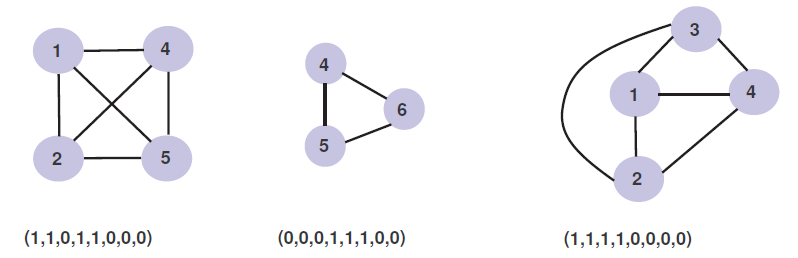
\includegraphics[scale=0.5]{figuras/Solucion/representacionSol}
%    \end{center}

%	$	
%	|\delta(\mathcal{C})| = \sum_{v \epsilon \mathcal{C}} deg(v) - |\mathcal{C}|\times|\mathcal{C}-1|$  
%	%\end{equation}	\Delta

\section{Resultados}
\subsection{Resultados I}
\begin{frame}\frametitle{Instancias de prueba}
\textbf{Caracterización instancias}
\begin{table}[h!]
	\hspace{-1cm}
	%\centering
	\scalebox{0.7}{  
	\begin{tabular}{l|rrrr}
		\hline
		{Instancias} & \multicolumn{4}{c}{Características de las instancias} \\
		%\cline{1-3} \cline{5-11} 
		 & $|V|$ & $|E|$ & Densidad & $|E(C)|$\\
		\hline
		c-fat200-1 	&200 	&1534	&0.071 	&81\\
		c-fat200-2 	&200 	&3235 	&0.163 	&306\\
		c-fat200-5 	&200 	&8473 	&0.426 	&1892\\
		c-fat500-1 	&500 	&4459 	&0.036 	&110\\
		c-fat500-2 	&500 	&9139 	&0.073 	&380\\
		c-fat500-5 	&500 	&23191 	&0.186 	&2304\\
		c-fat500-10 &500 	&46627 	&0.374 	&8930\\
		%p\_hat300-1	&300 	&10933	&0.244 	&789\\		
		p\_hat300-2 &300 	&21928 	&0.489 	&4637\\
		p\_hat300-3 &300 	&33390 	&0.744 	&7740\\
		%keller4 	&171 	&9435 	&0.649 	&1140\\
		keller5 	&776 	&225990 &0.752 	&15184\\
		%MANN\_a9 	&45 	&918 	&0.9273	&412\\
		MANN\_a27 	&378 	&70551 	&0.990 	&31284\\
		c125\_9 	&125 	&69632 	&0.899 	&236406\\	
		\hline
	\end{tabular}}	
\end{table}
\end{frame}

\subsection{Resultados II}
\begin{frame}\frametitle{Resultados obtenidos}
\begin{table}[h!]
	%\hspace{-1cm}
	\scalebox{0.7}{ 
	\begin{tabular}{l|rr|rr|r}
		\hline
		\multicolumn{1}{l}{} & \multicolumn{2}{c}{\textbf{GRASP/VND}} & \multicolumn{2}{l}{\textbf{Algoritmo Genético}} & GAP \\
		%\cline{1-3} \cline{5-11} 
		Instancias & $|E(C)|$ prom. & $T(s)$ prom. & $|E(C)|$ prom. & $T(s)$ prom. &(\%) \\
		\hline
		c-fat200-1 	&81 		&0.37 		&81 		&6.4	&0.0\\
		c-fat200-2 	&306 		&0.81 		&306 		&7.5	&0.0\\
		c-fat200-5 	&1892 		&4.94 		&1892 		&12.5	&0.0\\
		c-fat500-1 	&110 		&2.46 		&110 		&16.15	&0.0\\
		c-fat500-2 	&380 		&5.83 		&380 		&14.3	&0.0\\
		c-fat500-5 	&2304 		&10.85 		&2304 		&20.36	&0.0\\
		c-fat500-10 &8930 		&65.74 		&8930 		&32.59	&0.0\\
		p\_hat300-2 &4636.2 	&3659.39 	&4633.40 	&171.9	&$\approx$0.0\\
		p\_hat300-3 &7726.8 	&3992.42 	&7387.27 	&279.8	&0.04\\
		c125\_9 	&2766 		&253.25	 	&2737.2 	&5.0	&0.01\\
		keller5 	&15183.24 	&1167.64 	&12382 		&50.57	&0.18\\
		MANN\_a27 	&31244.10 	&548.54 	&30405 		&46.49	&0.03\\		
		\hline
	\end{tabular}}	
\end{table}
\end{frame}

\section{Conclusiones}
\begin{frame} \frametitle{Conclusiones}
\begin{block} {Conclusiones}
   	\begin{itemize} 
   	\begin{small}     	
	\item Aplicaciones diversas en diferentes áreas.
	\item Se demuestra la $\mathcal{NP}$-Completitud.
	\item Solución competitiva con las existentes y con tiempos de ejecución muy buenos.   	
	\end{small} 	
 	\end{itemize} 	
 \end{block}
\end{frame}

\subsection{Trabajo Futuro}
\begin{frame} \frametitle{Trabajo Futuro}
\begin{block} {Trabajo Futuro}
 	 \begin{itemize}
 	 	\item Aplicaciones reales en grandes superficies.
 	 	\item Explorar la versión con pesos en las aristas, (WMCC).
 	 \end{itemize}  
 \end{block} 	   
\end{frame}

\subsection{Gracias}
\begin{frame} \frametitle{Fin}
\begin{huge}
Gracias por su atención.
\end{huge}
\end{frame}